\documentclass[11pt,reqno]{amsart}

%%%%%%%%%%%%%%%%%%%%%%%%%%%%%%%%%%%%%%%%%%%%%%%%%%%
%								Packages									         %
%%%%%%%%%%%%%%%%%%%%%%%%%%%%%%%%%%%%%%%%%%%%%%%%%%%

\usepackage[T1]{fontenc}

\usepackage{amsmath}							
\usepackage{amssymb}
\usepackage{amsthm}
\usepackage{amscd}
\usepackage{amsfonts}
\usepackage{stmaryrd}
\usepackage{algorithm, algorithmic}
\usepackage{ wasysym }
\usepackage{caption}
\usepackage{subcaption}
\usepackage{euler}
\renewcommand{\rmdefault}{pplx}
\usepackage{extarrows}
\usepackage[colorlinks, linktocpage, citecolor = red, linkcolor = blue]{hyperref}
\usepackage{color}
\usepackage{tikz}									
\usepackage{fullpage}
\usepackage[shortlabels]{enumitem}

\linespread{1.1}

%%%%%%%%%%%%%%%%%%%%%%%%%%%%%%%%%%%%%%%%%%%%%%%%%%%
%								Theorems 								         %
%%%%%%%%%%%%%%%%%%%%%%%%%%%%%%%%%%%%%%%%%%%%%%%%%%%

\newtheorem{maintheorem}{Theorem}
\renewcommand*{\themaintheorem}{\Alph{maintheorem}}

\newtheorem{theorem}{Theorem}[section]
\newtheorem{lemma}[theorem]{Lemma}
\newtheorem{proposition}[theorem]{Proposition}
\newtheorem{corollary}[theorem]{Corollary} 
\newtheorem{conjecture}[theorem]{Conjecture} 

\theoremstyle{definition}
\newtheorem{maindefinition}[maintheorem]{Definition}								
\newtheorem{definition}[theorem]{Definition}
\newtheorem{question}[theorem]{Question}
\newtheorem{example}[theorem]{Example}
\newtheorem{construction}[theorem]{Construction}

%\theoremstyle{remark}
\newtheorem{remark}[theorem]{Remark}
\newtheorem{remarks}[theorem]{Remarks}
\newtheorem*{maintheorema}{Theorem \ref{thm:main}}


\renewcommand{\algorithmicrequire}{\textbf{Input:}}
\renewcommand{\algorithmicensure}{\textbf{Output:}}

%%%%%%%%%%%%%%%%%%%%%%%%%%%%%%%%%%%%%%%%%%%%%%%%%%%
%								Operators									         %
%%%%%%%%%%%%%%%%%%%%%%%%%%%%%%%%%%%%%%%%%%%%%%%%%%%


\newcommand{\madeline}[1]{{\color{purple} \sf  Madeline: [#1]}}

\newcommand{\R}{\mathbb{R}}
\newcommand{\C}{\mathbb{F}}
\newcommand{\F}{\mathbb{F}}
\newcommand{\nul}{\mathrm{null}}
\newcommand{\range}{\mathrm{range}}
\newcommand{\spa}{\mathrm{span}}



%%%%%%%%%%%%%%%%%%%%%%%%%%%%%%%%%%%%%%%%%%%%%%%%%%%
%                                                                          Title                                                                             %
%%%%%%%%%%%%%%%%%%%%%%%%%%%%%%%%%%%%%%%%%%%%%%%%%%%

\title{The Fundamental Theorem of Linear Maps}

\author[M. Brandt]{Madeline Brandt}
\address{Department of Mathematics, Brown University,  Providence, RI 02912}
\email{\href{mailto:madeline_brandt@brown.edu}{madeline\_brandt@brown.edu}}
\urladdr{\url{https://sites.google.com/view/madelinebrandt}}



%%%%%%%%%%%%%%%%%%%%%%%%%%%%%%%%%%%%%%%%%%%%%%%%%%%%%%

\begin{document}


\maketitle
\setcounter{tocdepth}{1}
%\tableofcontents

%%%%%%%%%%%%%%%%%%%%%%%%%%%%%%%%%%%%%%%%%%%%%%%%%%%%%%
\begin{abstract}
   Linear maps $T$ between two vector spaces $V$ and $W$ are a fundamental concept of linear algebra. In this paper, we introduce two subspaces one can associate to such a linear map. The first, called the \emph{null space of $T$}, is a subspace of $V$. The second, called the \emph{range of $T$}, is a subspace of $W$. The main result of this paper is that the dimension of $V$ is equal to the sum of the dimensions of the null space and the range of $T$. We give two applications of this result. The first gives a condition to determine when there are injective or surjective maps between $V$ and $W$. The second gives conditions for a system of homogeneous linear equations to have a nonzero solution.
\end{abstract}

%%%%%%%%%%%%%%%%%%%%%%%%%%%%%%%%%%%%%%%%%%%%%%%%%%%%%%
\section{Introduction}

Vector spaces and linear maps are fundamental objects of linear algebra, with applications across all of mathematics and the sciences. Let $V$ and $W$ be vector spaces over a field $\F$, with $V$ finite-dimensional, and let $T:V\rightarrow W$ be a linear map. In this paper, we introduce two subspaces one can associate to such a linear map. The first, called the \emph{null space of $T$}, is the the subspace $\nul(T)$ of $V$ consisting of all those vectors that are mapped to 0. 
The second, called the \emph{range of $T$}, is a subspace $\range(T)$ of $W$ consisting of all outputs of $T$. We study the following fundamental theorem about the relationship between the dimensions of these spaces.

\begin{maintheorem}[As stated in \cite{axler}]
\label{thm:main}
Suppose $V$ and $W$ are vector spaces, with $V$ finite-dimensional. Let $T: V \rightarrow W$ be a linear map. Then $\range(T)$ is finite dimensional, and 
$$
\dim V = \dim (\nul (T)) + \dim (\range (T)).
$$
\end{maintheorem}


\begin{example}
Let $T : \R^3 \rightarrow \R^3$ be the linear map defined by
$
T(x,y,z) = (0,0,z).
$
Then, the null space of $T$ is 
$
\nul(T) = \{(x,y,0) \in \R^3\}
$
and the range of $T$ is $\range(T) = \{(0,0,z) \in \R^3\}$. This is pictured in Figures \ref{fig:test1} and \ref{fig:test2}. We see in this case that $$\dim(\R^3) = 3  = 2+1 = \dim(\nul(T)) + \dim(\range(T)).$$
\begin{figure}[h]
\centering
\begin{minipage}{.5\textwidth}
  \centering
  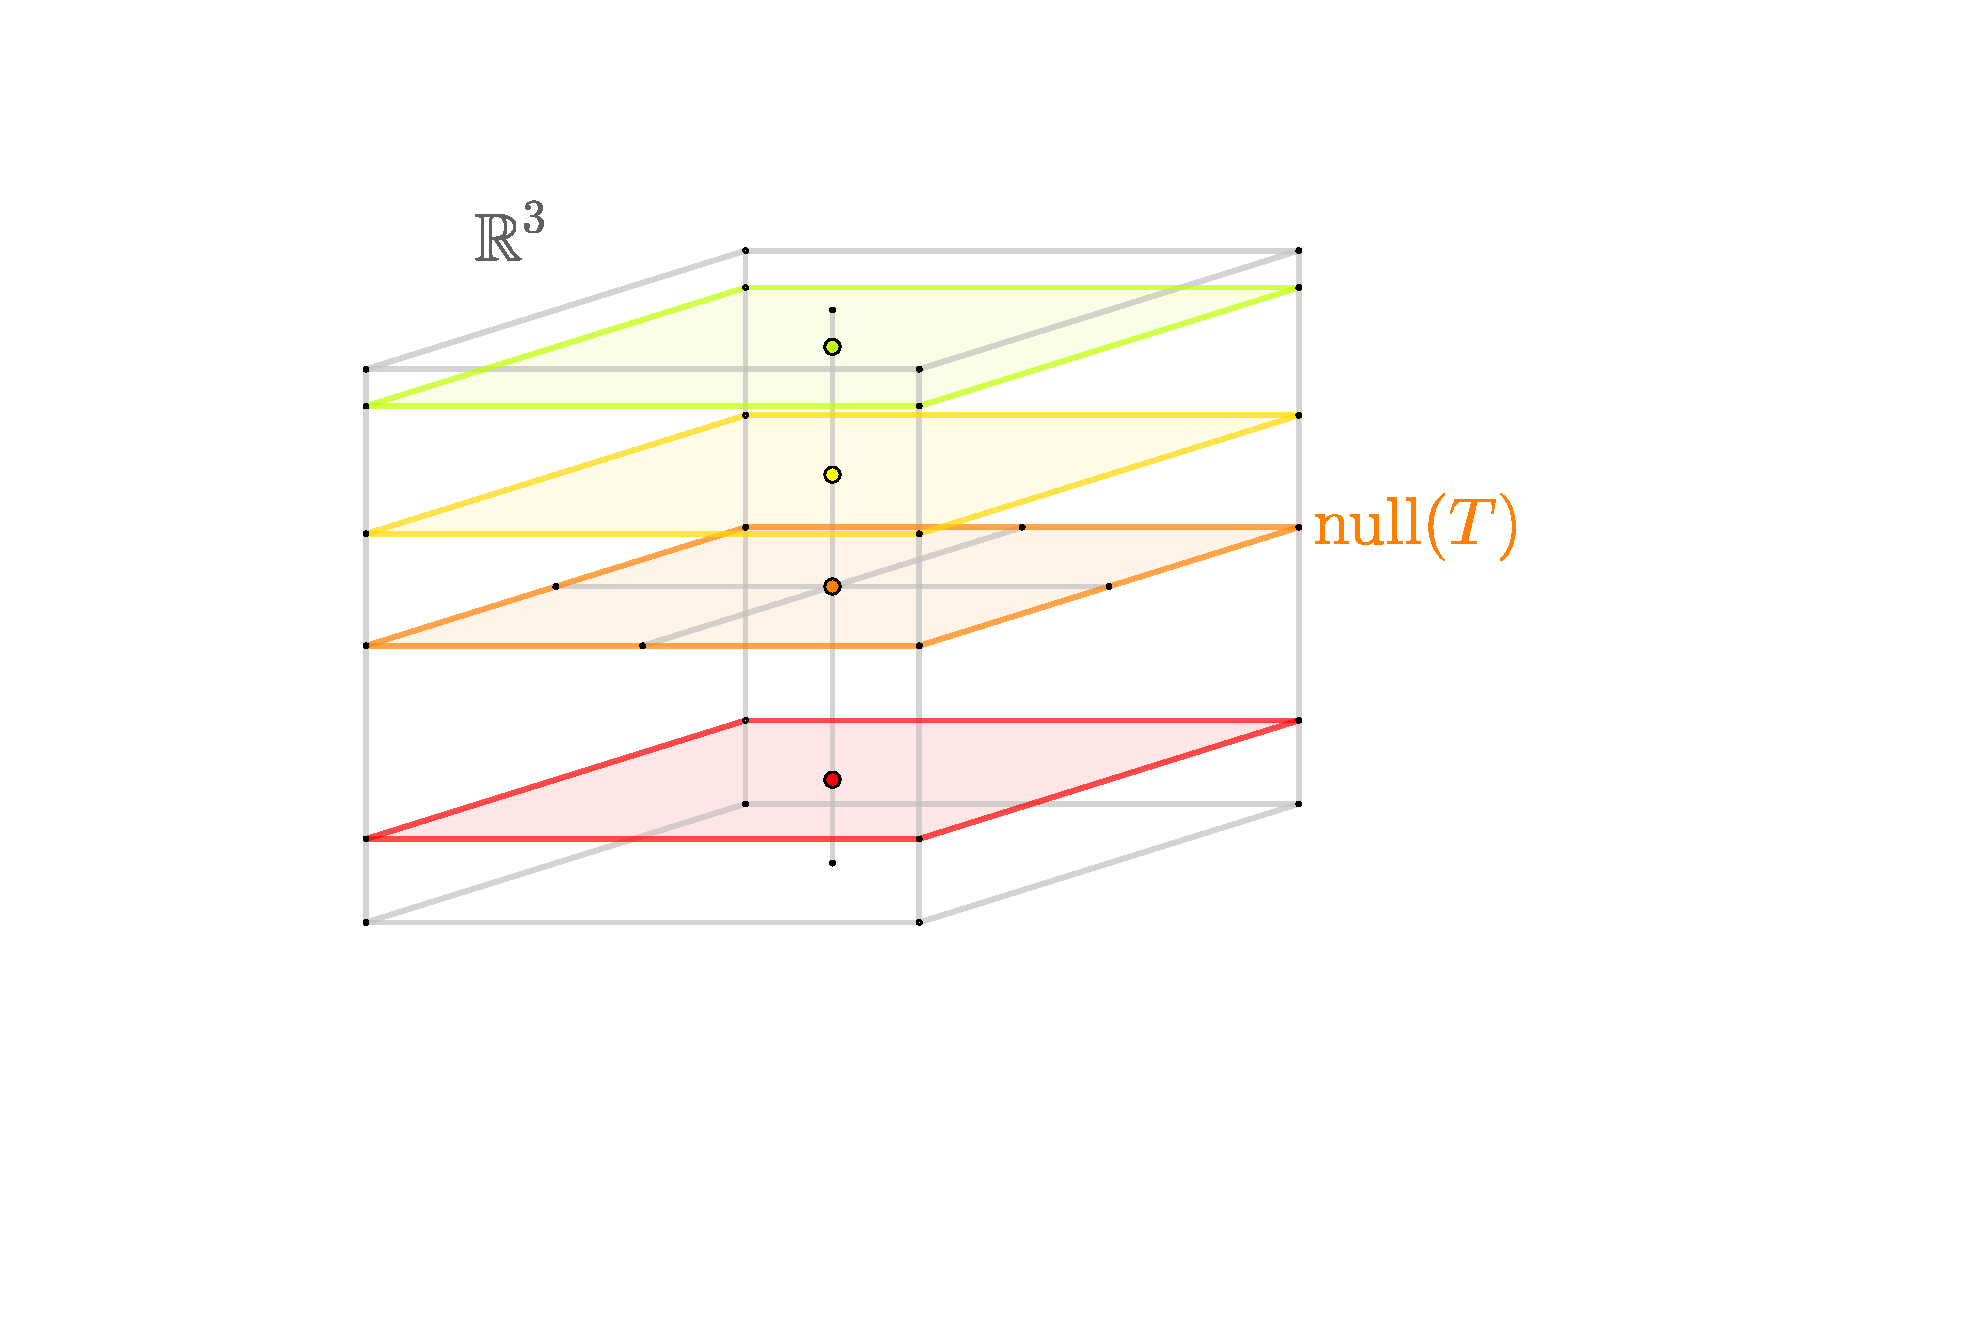
\includegraphics[height = 1.7 in]{nullT.pdf}
  \captionof{figure}{$\nul(T) \subset \R^3$.}
  \label{fig:test1}
\end{minipage}%
\begin{minipage}{.5\textwidth}
  \centering
  \includegraphics[height = 1.7 in]{rangeT.png}
  \captionof{figure}{$\range(T) \subset \R^3$.}
  \label{fig:test2}
\end{minipage}
\end{figure}
\end{example}

The history of Theorem \ref{thm:main} is complex. Historically, mathematicians were interested in solving systems of linear equations, which naturally led them to study determinants and matrices \cite{history}. In this context, the \emph{rank} of a determinant was defined by Frobenius in 1878 \cite{frobenius}. The first known use of the term \emph{rank} with regards to a matrix, which is equivalent to the rank of the associated linear map, is by Browmowich \cite{bromowich}. 
The \emph{nullity} of a square matrix was defined by Sylvester in 1884 \cite{history}. So, it is likely that by the 1880's some version of Theorem \ref{thm:main} had been formulated. Since the history of linear algebra is long, dating back to the Babylonians, and the notation and nomenclature is quite different from the modern formulation, it is extremely difficult to determine who Theorem \ref{thm:main} should be attributed to, and mathematical historians have not reached a consensus.

Mathematicians now view Theorem \ref{thm:main} as a special case of the first isomorphism theorem for algebra in the case of vector spaces. Even more abstractly, Theorem \ref{thm:main} can be viewed as a corollary of the splitting lemma from homological algebra. 

Theorem \ref{thm:main} is quite impactful. In this paper, we discuss one of the most important applications of Theorem \ref{thm:main}, which is that it guarantees solutions to systems of linear equations in certain situations. Systems of linear equations need to be solved in many situations across the sciences.
As another application, Theorem \ref{thm:main} also guarantees solutions to ordinary differential equations. 


The structure of the paper is as follows. In Section \ref{sec:background} we give the definitions of the null space and the range of a linear map, with examples. In Section \ref{sec:proof} we give the proof of Theorem \ref{thm:main}. Finally, in Section \ref{sec:applications}, we give two applications of Theorem \ref{thm:main}, showing that it can be used to determine when there can be injective or surjective maps between two vector spaces, and giving a condition for the existence to solutions of certain systems of linear equations. In Section \ref{sec:directions}, we give a few questions which could be studied to pursue the topic further.


\subsection*{Acknowledgements}
I would like to thank Sir Beanjamin Brandt Jr. for many discussions, for his insightful comments, and for providing useful feedback on an early version of this article.

%%%%%%%%%%%%%%%%%%%%%%%%%%%%%%%%%%%%%%%%%%%%%%%%%%%%%%
\section{Background}
\label{sec:background}

We assume the reader is familiar with the fundamentals of fields, vector spaces, and linear maps as in \cite[Chapters 1, 2, and 3a]{axler}. Throughout, let $\F$ be a field, and let $V$ and $W$ be vector spaces. We now follow \cite[Chapter 3b]{axler}.

Given a linear map $T:V\rightarrow W$, there are two natural vector spaces one may associate to $T$. One is a subspace of $V$ and is called the \emph{null space}. The other is a subspace of $W$ and is called the \emph{range}. Our main theorem, Theorem \ref{thm:main}, will relate the dimensions of these spaces. We define them as follows.

\begin{definition}
Let $T: V \rightarrow W$ be a linear map. Then the \emph{null space} of $T$, denoted $\nul(T)$, is the set
$$
\nul(T) = \{v \in V\ |\ T(v) = 0\}.
$$
The \emph{range} of $T$, denoted $\range(T)$, is the set
$$
\range(T) = \{T(v)\ |\ v \in V\}.
$$
\end{definition}

We now give some examples to illustrate what these sets are for some specific linear maps.

\begin{example}
\label{ex:1}
Suppose $T: V \rightarrow W$ is the 0 map. Then, $\nul(T) = V$ and $\range(T) = \{0\}$.
\end{example}

\begin{example}
\label{ex:2}
Suppose $S:\R^3 \rightarrow \R^2$ is defined by $S(x,y,z) = (x,y)$. Then, $\nul(S) = \{(0,0,z) \in \R^3\ |\ z\in \R\}$ and $\range(S) = \R^2$.
\end{example}


\begin{example}
\label{ex:3}
Suppose $R:\R^3 \rightarrow \R^2$ is defined by $R(x,y,z) = (x+y+z, x+y+z)$. Then, $\nul(R) = \{(x,y,z) \in \R^3\ |\ x+y+z=0\}$ and $\range(R) = \{(x,x)\in \R^2\ |\ x \in \R\}$.
\end{example}


Now, we show that both $\nul(T)$ and $\range(T)$ are vector spaces for any linear map $T:V \rightarrow W$.

\begin{proposition}
Suppose $T$ is a linear map from $V$ to $W$. Then $\nul(T)$ is a subspace of $V$ and $\range(T)$ is a subspace of $W$.
\end{proposition}

\begin{proof} 
First, we show that $\nul(T)$ is a subspace of $V$. To do this, we need to show that $\nul(T)$ satisfies the three subspace axioms:
\begin{enumerate}
    \item Contains 0: We know $T(0) = 0$, so $0 \in \nul(T)$.
    \item Closed under addition: Suppose $u,v \in \nul(T)$. Then:
    $$
   T(u + v) = T(u) + T(v) = 0 + 0 = 0
    $$
    so $u+ v \in \nul(T)$.
    \item Closed under scalar multiplication: Suppose $u \in \nul(T),$ and $\lambda \in \F$. Then
    $$
    T(\lambda u) = \lambda T(u) = \lambda 0 = 0,
    $$
    so $\lambda u \in \nul T$.
\end{enumerate}
Now, we show that $\range(T)$ is a subspace of $W$. To do this, we need to show that $\range(T)$ satisfies the three subspace axioms:
\begin{enumerate}
   \item Contains 0: $T(0) = 0$, so $0$ is in the range of $T$.
    \item Closed under addition: Let $T(v)$ and $T(w) \in \range(T)$ for some $v,w \in V$. Then $T(v) + T(w) = T(v+w)$, so $T(v) + T(w) \in \range(T)$.
    \item Closed under scalar multiplication: If $T(v)\in \range(T)$ and $\lambda \in \F$, then $\lambda T(v) = T(\lambda v)$, so we have that $\lambda T(v) \in \range(T)$.
\end{enumerate}
This completes the proof.
\end{proof}




%%%%%%%%%%%%%%%%%%%%%%%%%%%%%%%%%%%%%%%%%%%%%%%%%%%%%%
\section{Main Theorem}
\label{sec:proof}

Now that we have introduced the null space and the range of a linear map, we are ready to state and prove Theorem \ref{thm:main}. This theorem says that the sum of the dimensions of the null space and the range equal the dimension of the domain of the linear map.

\begin{maintheorema}[{Fundamental Theorem of Linear Maps, \cite[3.22]{axler}}]
Suppose $V$ and $W$ are vector spaces, with $V$ finite-dimensional. Let $T: V \rightarrow W$ be a linear map. Then $\range(T)$ is finite dimensional, and 
$$
\dim V = \dim (\nul (T)) + \dim (\range (T)).
$$
\end{maintheorema}

We follow the proof given in \cite[3.22]{axler}.

\begin{proof}
Let $u_1, \ldots, u_m$ be a basis of $\null(T)$ so that $\dim (\null(T)) = m$. We can extend the list $u_1, \ldots, u_m$ to be a basis
$$
u_1, \ldots, u_m, v_1, \ldots, v_n
$$
of $V$ by \cite[2.33]{axler}. Then, we have $\dim(V) = m+n$. We will show that $T(v_1), \ldots, T(v_n)$ is a basis of $\range(T)$, and this will show that $\range(T)$ is finite dimensional with $\dim (\range(T)) = n$, completing the proof.

First, we show that $T(v_1), \ldots, T(v_n)$ spans $\range(T)$. Let $v \in V$. Then, we may write
$$
v = a_1 u_1 + \cdots + a_mu_m + b_1 v_1 + \cdots + b_nv_n
$$
for scalars $a_1,\ldots, a_m, b_1,\ldots, b_n \in \F$. Then,
\begin{align*}
    T(v) &= T( a_1 u_1 + \cdots + a_mu_m + b_1 v_1 + \cdots + b_nv_n) \\
    &= a_1 T(u_1) + \cdots a_mT(u_m) + b_1 T(v_1) + \cdots + b_n T(v_n) \\
    &= 0 + \cdots + 0 + b_1 T(v_1) + \cdots + b_n T(v_n) \\
    &=  b_1 T(v_1) + \cdots + b_n T(v_n).
\end{align*}
Thus, $T(v_1), \ldots, T(v_n)$ spans $\range(T)$, so $\range(T)$ is finite-dimensional.

Now, it remains to show that $T(v_1), \ldots, T(v_n)$ is linearly independent. For this, suppose for some scalars $c_1, \ldots, c_n \in \F$ we have
$$
c_1T(v_1)+ \cdots +  c_nT(v_n) = 0.
$$
Then, we have that $T(c_1 v_1 + \cdots + c_n v_n) = 0$ so that $c_1 v_1 + \cdots + c_n v_n \in \nul(T)$. Since $u_1, \ldots, u_m$ spans $\nul(T)$, we can write
$$
c_1 v_1 + \cdots + c_n v_n = d_1 u_1 + \cdots + d_m u_m.
$$
But, since $u_1, \ldots, u_m, v_1, \ldots, v_n$ is a linearly independent set, we must have that $c_1 = \cdots = c_n = d_1 = \cdots = d_m = 0$. Thus, $T(v_1), \ldots, T(v_n)$ is linearly independent, and the proof is complete.
\end{proof}

We now return to the examples from Section \ref{sec:background} to illustrate Theorem \ref{thm:main}.

\begin{example}
Consider Examples \ref{ex:1}, \ref{ex:2}, and \ref{ex:3} of linear maps from $\R^3$ to $\R^2$. We observe that in these examples, the dimension of the range and the dimension of the null space sum to 3, see Table \ref{tab:ex}.

\begin{table}[h]
    \centering
    \begin{tabular}{c|c | c | c}
    map & dimension of null space & dimension of range & total \\
    \hline
 $T$ & 3 & 0 & 3 \\
 $S$ & 1 & 2 & 3 \\
 $R$ & 2 & 1 & 3
    \end{tabular}
    \caption{The maps in Examples \ref{ex:1}, \ref{ex:2}, and \ref{ex:3} satisfy Theorem \ref{thm:main}.}
    \label{tab:ex}
\end{table}
\end{example}


%%%%%%%%%%%%%%%%%%%%%%%%%%%%%%%%%%%%%%%%%%%%%%%%%%%%%%
\section{Applications}
\label{sec:applications}

We now give two applications that demonstrate the utility of Theorem \ref{thm:main}.

\subsection{Existence of injective and surjective linear maps}

As a corollary of Theorem \ref{thm:main}, one can determine whether or not there exist surjective or injective linear maps from $V$ to $W$ by examining the dimension of the spaces $V$ and $W$.

\begin{corollary}[{\cite[3.24]{axler}}]
Suppose $V$ and $W$ are finite-dimensional vector spaces such that $\dim (V) < \dim (W)$. Then no linear map from $V$ to $W$ is surjective.
\end{corollary}
\begin{proof}
Let $T$ be a linear map from $V$ to $W$. Then, by Theorem \ref{thm:main}, we have
\begin{align*}
    \dim(\range(T)) &= \dim(V) - \dim(\nul(T))\\
    & \leq \dim (V) \\
    & < \dim (W).
\end{align*}
This implies that the range of $T$ cannot be all of $W$. Thus, there is no surjective linear map from $V$ to $W$.
\end{proof}


\begin{corollary}[{\cite[3.23]{axler}}]
\label{cor:noinj}
Suppose $V$ and $W$ are finite-dimensional vector spaces such that $\dim (V) > \dim (W)$. Then no linear map from $V$ to $W$ is injective.
\end{corollary}
\begin{proof}
Let $T$ be a linear map from $V$ to $W$. Suppose for contradiction that $T$ is injective. Then, $\dim(\nul(T)) = 0$. Then, by Theorem \ref{thm:main}, we have
\begin{align*}
    \dim(V) &= \dim(\range(T)) + \dim(\nul(T)) \\
    &= \dim(\range(T)) + 0 \\
    &\leq \dim(W).
\end{align*}
But, this contradicts the assumption that $\dim(V) > \dim(W)$. Thus, there is no injective linear map from $V$ to $W$.
\end{proof}


\subsection{Solutions to systems of equations}

Theorem \ref{thm:main} can also be used to determine whether or not a system of linear equations has a nonzero solution. Let $m$ and $n$ be positive integers, and let $A_{j,k} \in \F$ for $j = 1,\ldots,m$ and $k=1,\ldots, n$. Consider the system of linear equations 
\begin{equation}
\label{eqn:linearsystem}
    \sum_{k = 1}^n A_{1,k} x_k = 0, \ \ 
    \cdots ,\ \ 
    \sum_{k = 1}^n A_{m,k} x_k = 0.
\end{equation}
Clearly, a solution to this system of equations would be $x_1 = \cdots = x_n = 0$. When do there exist non-zero solutions to this system of equations?

We now re-frame this question to be one about linear maps, so that we can apply Theorem \ref{thm:main}. Define a linear map $T: \F^n \rightarrow \F^m$ by
$$
T(x_1, \ldots, x_n) = \left( \sum_{k = 1}^n A_{1,k} x_k , \ \ 
    \cdots ,\ \ 
    \sum_{k = 1}^n A_{m,k} x_k  \right).
$$
In this setup, the equation $T(x_1, \ldots, x_n ) = 0$ is equivalent to the system in Equation \ref{eqn:linearsystem}. Therefore, we can rephrase the question as when does the null space of $T$ contain more than just $0$?
\begin{corollary}[{\cite[3.26]{axler}}]
A system of linear equations as in Equation \ref{eqn:linearsystem} with more variables than equations has nonzero solutions.
\end{corollary}
\begin{proof}
If there are more variables than equations, then we have a linear map $T: \F^n \rightarrow \F^m$ with $n>m$. By Corollary \ref{cor:noinj}, this implies that $T$ is not injective, thus $\nul(T) \not = \{0\}$. Hence, there is a nonzero element of $\nul(T)$, and this is a nonzero solution to the system of equations.
\end{proof}


%%%%%%%%%%%%%%%%%%%%%%%%%%%%%%%%%%%%%%%%%%%%%%%%%%%%%%
\section{Future directions}
\label{sec:directions}

In this section, we give some directions for future study.

\begin{question}
Is there an analogue of Theorem \ref{thm:main} for infinite-dimensional vector spaces? 
\end{question}
In order to answer this question, we would need to make sense of how to quantify the dimension of an infinite-dimensional vector space, and how to add infinite numbers.

\begin{question}
Given a linear map $T: V \rightarrow W$, we can write the matrix of the linear map $M(T)$. Is there a way to quantify $\dim(\null(T))$ and $\dim(\range(T))$ in terms of the matrix $M(T)$ to obtain a version of Theorem \ref{thm:main} for matrices? 
\end{question}




%%%%%%%%%%%%%%%%%%%
\bibliographystyle{abbrv}
\bibliography{sample}

\end{document}



